\section{Engine}

The program core is as simple as it could be. It consists of two threads within a process - one thread for GUI and one thread for computation part. The main principle of thread dependency is presented on Fig. \ref{Fig:threads}. When the GUI thread exits, an exit event is set to true, causing the parent process to terminate.

\begin{figure}
\centering
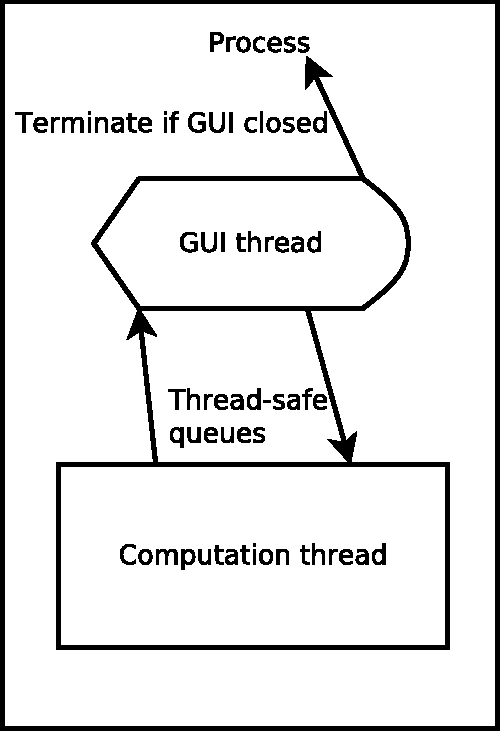
\includegraphics[scale=0.6]{figures/threads}

\caption[Threads scheme]{\label{Fig:threads}Threading structure in project}
\end{figure}

The classes (Fig. \ref{Fig:classes}) are used to ensure data consistency. The classes \textit{mri\_struct} and \textit{mri\_diff} are used to hold the actual data, read and parsed with the reading \textit{mri\_read(filename)} function and a class constructor. Classes \textit{simens\_communicator} and \textit{simens\_msg} are useful for communication between the processes and maintaining the windowed app execution control.

\begin{figure}
\centering
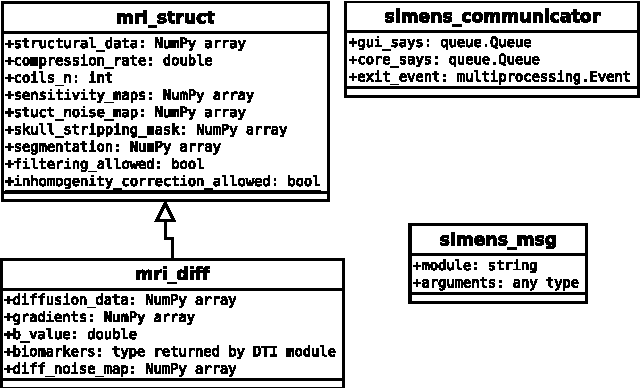
\includegraphics[scale=1]{figures/classes}

\caption[Classes scheme]{\label{Fig:classes}Custom classes used in project}
\end{figure}

The data flow complies with the one shown on the Fig. \ref{fig:figures/drzewo}. It has been achieved by sending appropriate messages through the communication queues. The meritorical correctness of the performed operations is ensured by graying out GUI buttons. That being said, the user is unable to perform an action which is not meritorically correct.